% % % % % % % % % % % % % % % % % % % % % % % % % % % % % % % % % %
%  Devolutiva — Fase 1: Imersão
%  Disciplina: Design Thinking (DE_233) — ETE Cícero Dias
%  Profa. Samara Silva  ·  Recife, 28 de junho de 2026
% % % % % % % % % % % % % % % % % % % % % % % % % % % % % % % % % %

\documentclass[
  sigconf,
  nonacm, % Remove o rodapé da ACM
  language=portuguese
]{acmart}

% ── Desliga rodapé ACM ──────────────────────────────────────
\settopmatter{printacmref=false}
\setcopyright{none}
\acmYear{2026}
\let\balance\relax

% ── Mata a página temporária da ACM (compilação única via API) ──
\makeatletter
\def\acm@addtemp@page{}
\makeatother

% ── Pacotes ─────────────────────────────────────────────────
\usepackage[portuguese]{babel}
\usepackage{microtype}
\usepackage{booktabs}
\usepackage{tabularx}
\usepackage{array}
\usepackage{colortbl}
\usepackage[dvipsnames,table]{xcolor}
\usepackage[inline]{enumitem}
\usepackage{graphicx}
\usepackage{adjustbox}
\usepackage{fancyhdr}
\usepackage{eso-pic} % Para a capa preencher toda a página sem gerar páginas em branco

% ── Ajuste contra quebras de texto ruins (Textos Cortados) ──
\tolerance=1000
\emergencystretch=1.5em

% ── Cores ───────────────────────────────────────────────────
\definecolor{cgood}{HTML}{1E6B3A}
\definecolor{cwarn}{HTML}{8B4500}
\definecolor{cred}{HTML}{C0392B}
\definecolor{cmuted}{HTML}{666666}
\definecolor{crow}{HTML}{F2EFEB}

% ── Colunas customizadas para tabela ────────────────────────
\newcolumntype{L}[1]{>{\raggedright\arraybackslash}p{#1}}
\newcolumntype{C}[1]{>{\centering\arraybackslash}p{#1}}

% ── Comando nota destacada ───────────────────────────────────
\newcommand{\notadestaque}[2]{%
  \noindent\textbf{Nota:}\enspace%
  {\large\bfseries\color{cred}#1\,/\,#2\,pts}%
}

% ── Comando label de status ──────────────────────────────────
\newcommand{\statusok}[1]{{\small\bfseries\color{cgood}#1}}
\newcommand{\statuswarn}[1]{{\small\bfseries\color{cwarn}#1}}

% ── Renomeações PT-BR ────────────────────────────────────────
\AtBeginDocument{%
  \renewcommand{\abstractname}{Resumo}
  \renewcommand{\figurename}{Figura}
  \renewcommand{\tablename}{Tabela}
}

% ────────────────────────────────────────────────────────────
\begin{document}

% ── CAPA ────────────────────────────────────────────────────
\thispagestyle{empty}
\AddToShipoutPictureBG*{%
  \AtPageLowerLeft{%
    \IfFileExists{capa.png}{%
      
\includegraphics[width=\paperwidth,height=\paperheight]{capa.png}%
    }{%
      \IfFileExists{../../capa.png}{%
        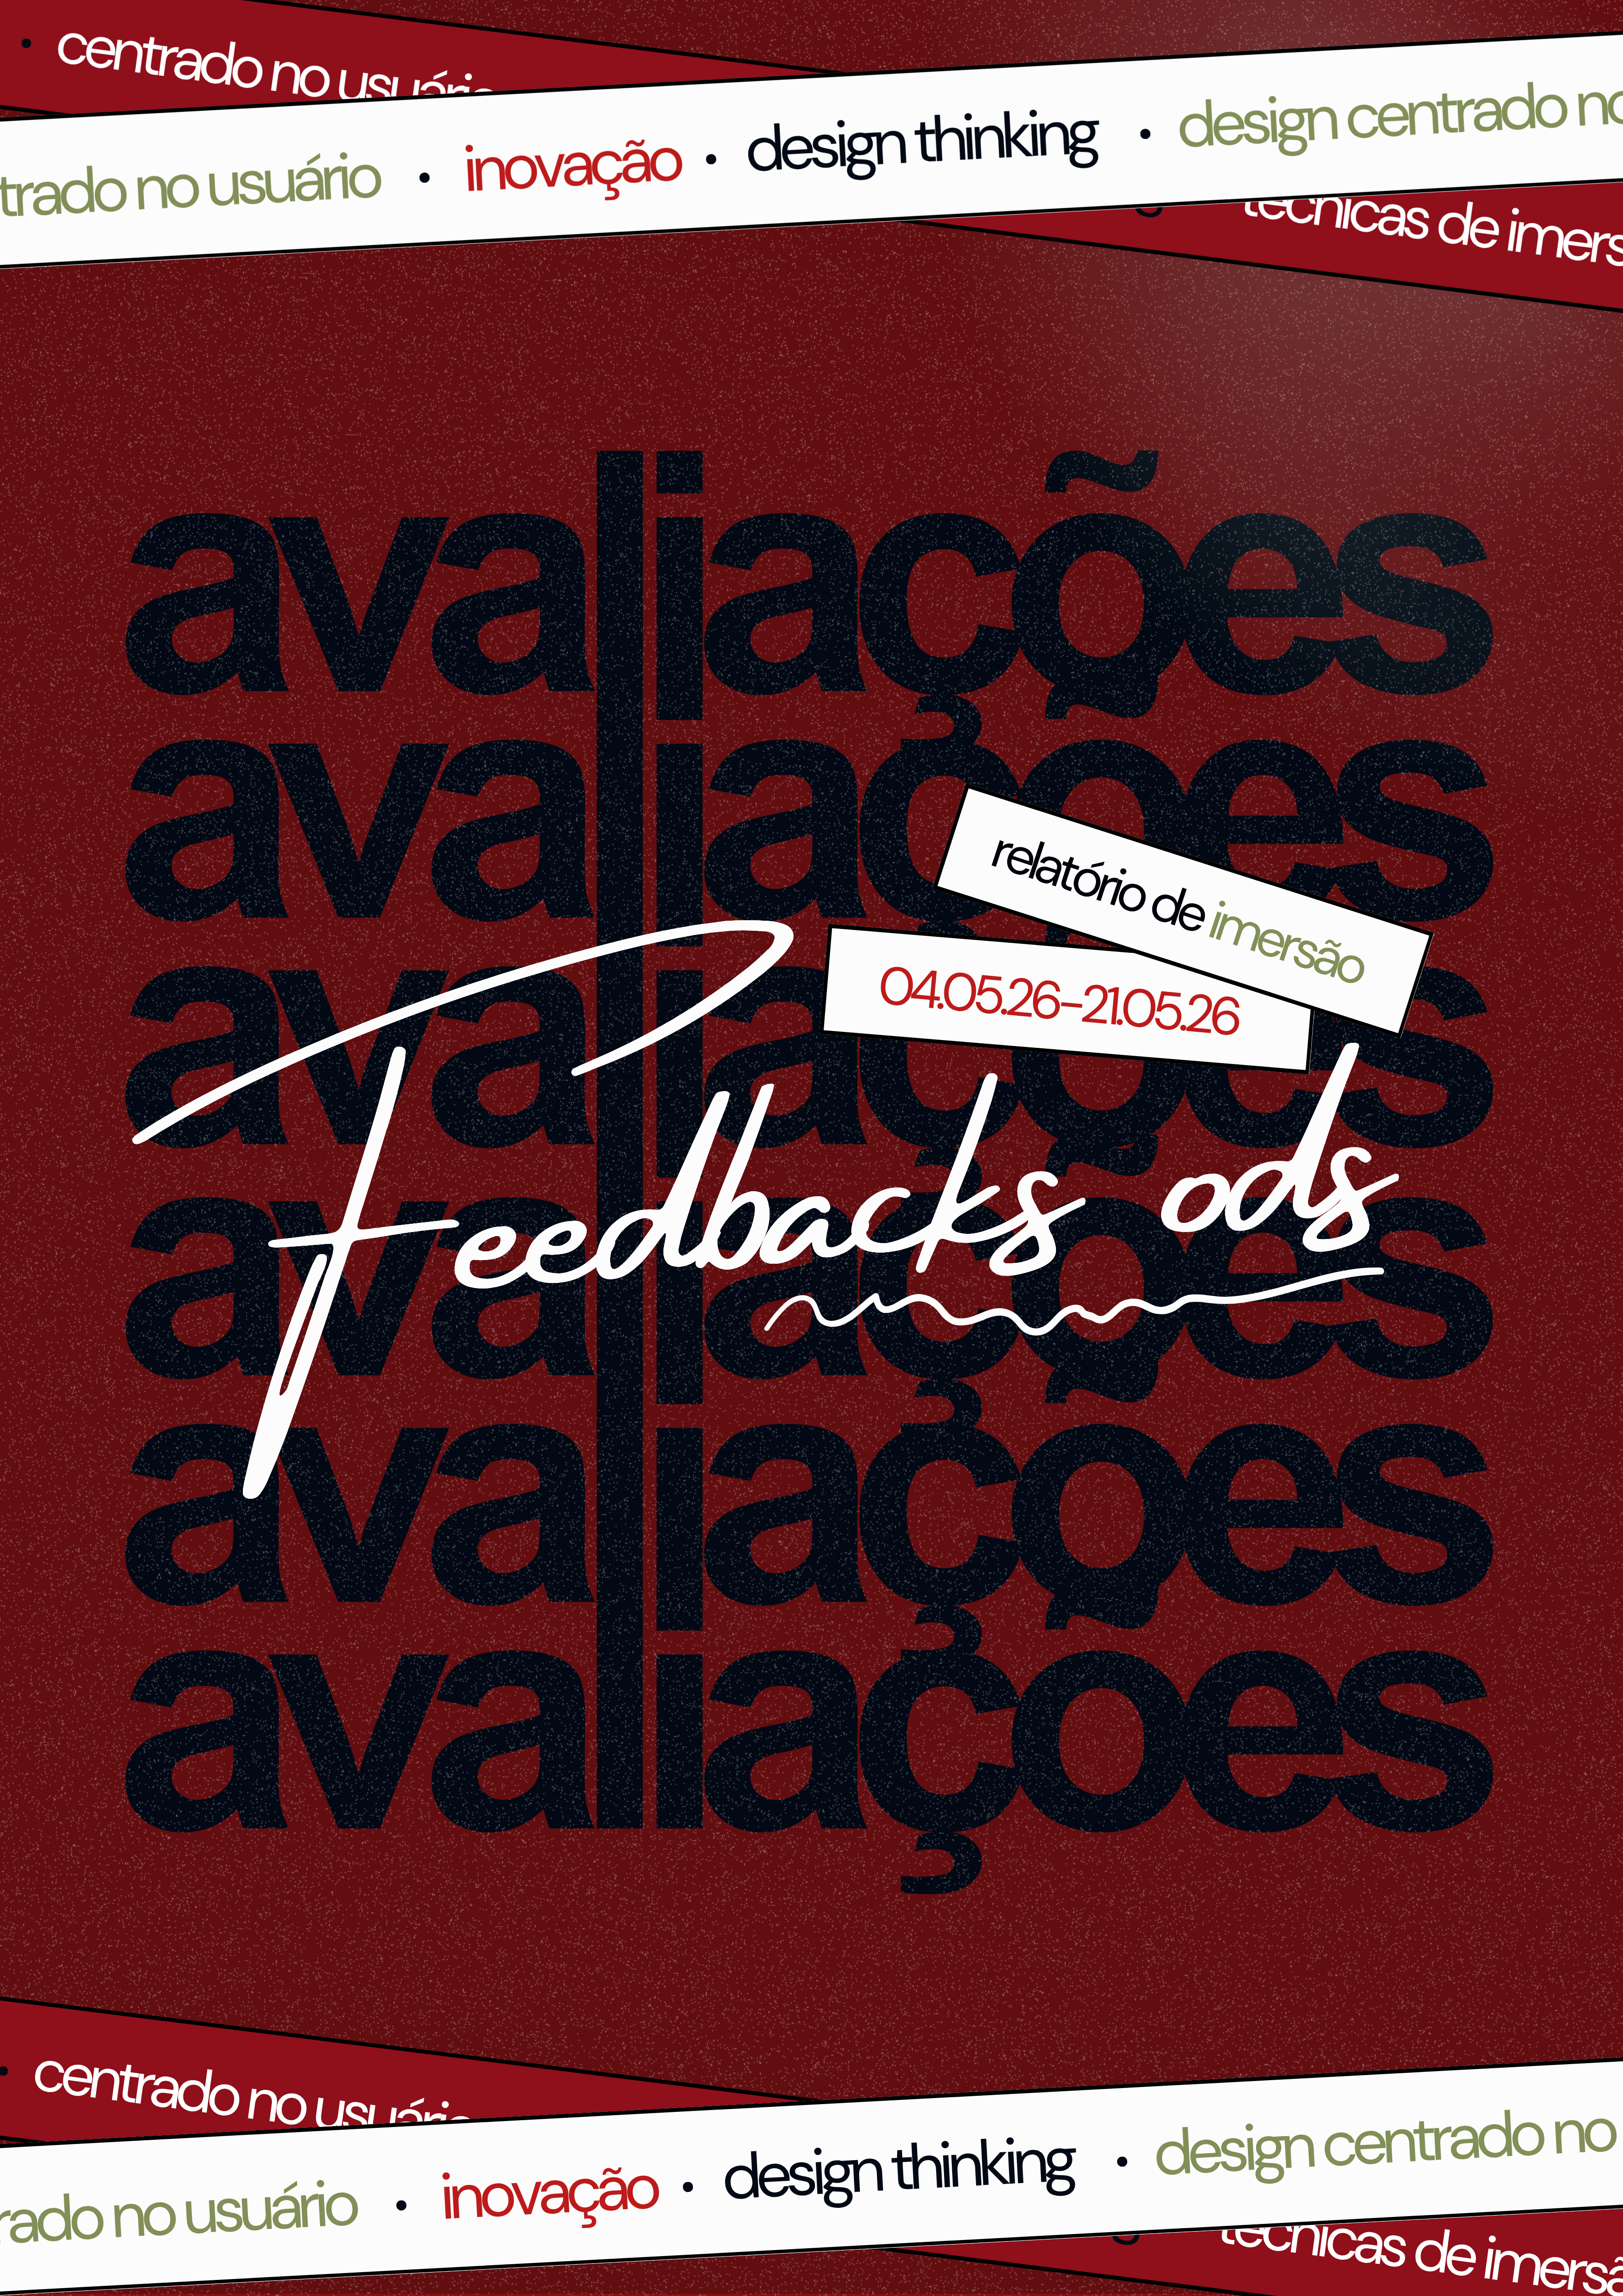
\includegraphics[width=\paperwidth,height=\paperheight]{../../capa.png}%
      }{%
        \parbox[b][\paperheight]{\paperwidth}{%
          \vspace*{10cm}\begin{center}{\large\color{gray}[capa.png não encontrada]}\end{center}%
        }%
      }%
    }%
  }%
}
\mbox{} % Caixa vazia para garantir que a página da capa seja gerada e preenchida
\clearpage

% ── CONFIGURAÇÃO DE PÁGINA PÓS-CAPA ─────────────────────────
\setcounter{page}{1}
\pagestyle{fancy}
\fancyhf{}
\renewcommand{\headrulewidth}{0pt}
\fancyfoot[C]{\thepage}
\setlength{\headsep}{0.8cm} % Distancia o cabeçalho do conteúdo das colunas

% ── METADADOS ────────────────────────────────────────────────
\title{Feedback Avaliativo de Projeto: Design Thinking --- Avaliação Completa}

\author{Profa.\ Samara Silva}
\authornote{Grupo: \textbf{Grupo 05 - Poluição Plástica} \textperiodcentered\ Per\'{i}odo: 22 de maio de 2026 \textperiodcentered\ Avaliado em: 28 de junho de 2026.}
\email{samarasilvia.educa@gmail.com}
\affiliation{%
  \institution{ETE C\'{i}cero Dias}
  \department{M\'{o}dulo 1 --- Turma A · 2026.1}
  \city{Recife}
  \state{Pernambuco}
  \country{Brasil}
}

\author{Grupo 05 - Poluição Plástica}
\affiliation{%
  \institution{ETE C\'{i}cero Dias}
  \department{Turma --- Turma A · 2026.1}
  \city{Recife}
  \state{Pernambuco}
  \country{Brasil}
}
\maketitle

\vspace{1em}
\section{Avaliação — Design Thinking}

\notadestaque{6,85}{11,00}

A seguir o detalhamento por fase da disciplina.

\subsection{Fase 1 — Imersão}

\notadestaque{2,47}{3,00}

\subsubsection*{Resumo dos Critérios}

\rowcolors{2}{crow}{white}
\begin{tabular}{@{} L{2.6cm} C{2.5cm} C{1.1cm} C{1.1cm} @{}}
\toprule
\textbf{Critério} & \textbf{Status} & \textbf{Nota} & \textbf{Máx.} \\
\midrule
Pesquisa Desk & \statusok{Completo} & \textbf{0,50} & 0,50 \\
Matriz de Alinhamento & \statusok{Completo} & \textbf{0,50} & 0,50 \\
Matriz CSD \& Perguntas de pesquisa & \statuswarn{Completo c/ ressalvas} & \textbf{0,42} & 0,50 \\
Pesquisa Primária & \statuswarn{Completo, mas inadequado} & \textbf{1,05} & 1,50 \\
\midrule
\textbf{Total} & & \textbf{\color{cred}2,47} & \textbf{3,00} \\
\bottomrule
\end{tabular}

\subsubsection*{Comentários}

\subsection{Pesquisa Desk}

\noindent\statusok{0,50\,/\,0,50 pts · Completo}

\begin{itemize}[leftmargin=14pt,itemsep=1pt,topsep=3pt,parsep=0pt]
  \item[\textcolor{cgood}{$\checkmark$}] {\small\textcolor{cgood}{Dados secundários relevantes e atuais sobre o ODS escolhido}}
  \item[\textcolor{cgood}{$\checkmark$}] {\small\textcolor{cgood}{Fontes confiáveis: ONU, IBGE, artigos acadêmicos ou jornalísticos}}
  \item[\textcolor{cgood}{$\checkmark$}] {\small\textcolor{cgood}{Contextualiza o problema com base factual}}
  \item[\textcolor{cgood}{$\checkmark$}] {\small\textcolor{cgood}{Conexão clara entre os dados e o problema}}
  \item[\textcolor{cgood}{$\checkmark$}] {\small\textcolor{cgood}{Coerência entre a CSD e o que foi pesquisado}}
  \item[\textcolor{cgood}{$\checkmark$}] {\small\textcolor{cgood}{Mínimo de 5 referências/links, esperado 8, ideal de 15 para cima}}
\end{itemize}

\subsection{Matriz de Alinhamento}

\noindent\statusok{0,50\,/\,0,50 pts · Completo}

\begin{itemize}[leftmargin=14pt,itemsep=1pt,topsep=3pt,parsep=0pt]
  \item[\textcolor{cgood}{$\checkmark$}] {\small\textcolor{cgood}{Identifica claramente quem é afetado pelo problema}}
  \item[\textcolor{cgood}{$\checkmark$}] {\small\textcolor{cgood}{Define o que o grupo pretende descobrir durante a imersão}}
  \item[\textcolor{cgood}{$\checkmark$}] {\small\textcolor{cgood}{As técnicas de imersão escolhidas são coerentes com os objetivos da pesquisa}}
  \item[\textcolor{cgood}{$\checkmark$}] {\small\textcolor{cgood}{Delimita adequadamente o que está dentro do escopo do projeto}}
  \item[\textcolor{cgood}{$\checkmark$}] {\small\textcolor{cgood}{Delimita adequadamente o que está fora do escopo do projeto}}
  \item[\textcolor{cgood}{$\checkmark$}] {\small\textcolor{cgood}{Apresenta uma hipótese inicial de solução relacionada ao problema investigado}}
  \item[\textcolor{cgood}{$\checkmark$}] {\small\textcolor{cgood}{Os resultados esperados da imersão são claros e coerentes com os objetivos da pesquisa}}
  \item[\textcolor{cgood}{$\checkmark$}] {\small\textcolor{cgood}{Há coerência entre os diferentes campos da matriz (problema, público, escopo, pesquisa e solução)}}
  \item[\textcolor{cgood}{$\checkmark$}] {\small\textcolor{cgood}{Preenchida com respostas, impressões ou perguntas reais do grupo sobre o problema}}
  \item[\textcolor{cgood}{$\checkmark$}] {\small\textcolor{cgood}{Linguagem clara e coerente, facilitando a compreensão das intenções do grupo}}
  \item[\textcolor{cgood}{$\checkmark$}] {\small\textcolor{cgood}{Serviu de base para planejar a pesquisa primária}}
\end{itemize}

\subsection{Matriz CSD \& Perguntas de pesquisa}

\noindent\statuswarn{0,42\,/\,0,50 pts · Completo c/ ressalvas}

\begin{itemize}[leftmargin=14pt,itemsep=1pt,topsep=3pt,parsep=0pt]
  \item[\textcolor{cgood}{$\checkmark$}] {\small\textcolor{cgood}{Os três quadrantes preenchidos: Certezas, Suposições, Dúvidas}}
  \item[\textcolor{cgood}{$\checkmark$}] {\small\textcolor{cgood}{Reflete o que o grupo sabe e precisa descobrir sobre o problema e seu contexto}}
  \item[\textcolor{cgood}{$\checkmark$}] {\small\textcolor{cgood}{Conteúdo específico do projeto — não genérico}}
  \item[\textcolor{cgood}{$\checkmark$}] {\small\textcolor{cgood}{Revela pensamento crítico}}
  \item[\textcolor{cgood}{$\checkmark$}] {\small\textcolor{cgood}{O quadrante de CERTEZAS expõe informações comprovadas ou confirmadas sobre o problema}}
  \item[\textcolor{cgood}{$\checkmark$}] {\small\textcolor{cgood}{Os itens do quadrante de CERTEZA estão relacionados diretamente ao contexto e ao público afetado}}
  \item[\textcolor{cgood}{$\checkmark$}] {\small\textcolor{cgood}{O quadrante de SUPOSIÇÕES expõe Informações que o grupo acha que são verdadeiras, mas ainda não comprovou}}
  \item[\textcolor{cgood}{$\checkmark$}] {\small\textcolor{cgood}{Os itens do quadrante de SUPOSIÇÃO demonstram reflexão sobre possíveis causas, comportamentos ou necessidades}}
  \item[\textcolor{cgood}{$\checkmark$}] {\small\textcolor{cgood}{O quadrante de DÚVIDAS expõem perguntas que o grupo precisa responder na pesquisa ou imersão como um todo}}
  \item[\textcolor{cgood}{$\checkmark$}] {\small\textcolor{cgood}{Os itens do quadrante de DÚVIDAS representam lacunas reais de conhecimento}}
  \item[\textcolor{cgood}{$\checkmark$}] {\small\textcolor{cgood}{O conteúdo da matriz está focado no problema investigado e não apenas no tema ou na ODS}}
  \item[$\square$] {\small\textcolor{cmuted}{Perguntas de Pesquisas formuladas como objetivos que norteiam o projeto geral}}
  \item[\textcolor{cgood}{$\checkmark$}] {\small\textcolor{cgood}{Deve se ter um mínimo de 5 itens no quadrante de certezas, suposições e dúvidas}}
\end{itemize}

Há um desvio metodológico importante na etapa de planejamento das perguntas de pesquisa que precisa ser corrigido: \textbf{houve uma sobreposição entre as Perguntas de Pesquisa e o Roteiro/Formulário do usuário. }Para o rigor acadêmico e prático do Design de Serviços/Produtos, é fundamental distinguir estas três camadas:

\begin{itemize}[leftmargin=14pt,itemsep=2pt,topsep=4pt]
  \item \textbf{Dúvidas (Matriz CSD):} Representam as incertezas internas do grupo. É o levantamento bruto do que a equipe não sabe. ex:\textit{"Os estudantes preferem estudar pelo celular ou pelo notebook?"}
  \item \textit{"Eles ainda têm o costume de usar agenda de papel?"}
  \item \textit{"Quanto tempo eles conseguem focar antes de pegar o celular?"}
\end{itemize}

\begin{itemize}[leftmargin=14pt,itemsep=2pt,topsep=4pt]
  \item \textbf{Perguntas de Pesquisa:} São os objetivos da investigação. Elas guiam o \textit{projeto} e a \textit{equipe}, sintetizando as dúvidas e suposições da CSD em grandes eixos investigativos. \textbf{Essas perguntas não devem ser feitas diretamente ao usuário. }ex:\textit{"Quais são os principais métodos e ferramentas de organização utilizados por universitários hoje, e quais são os maiores gatilhos comportamentais de distração durante o estudo?"}
\end{itemize}

\begin{itemize}[leftmargin=14pt,itemsep=2pt,topsep=4pt]
  \item \textbf{Roteiro/Formulário de Pesquisa:} É o instrumento de coleta. Aqui, as perguntas de pesquisa são traduzidas para a linguagem do usuário, de forma conversacional e empática, para evitar vieses. ex:\textit{"Você poderia me contar como costuma se organizar quando tem uma semana cheia de provas?"}
  \item \textit{"Lembre da última vez que você sentou para estudar e acabou perdendo o foco. Como foi isso? O que acabou tirando a sua atenção?"}
\end{itemize}

\textbf{O impacto desse erro:} Em vez de definirem os eixos estratégicos que o projeto precisa investigar, a equipe inseriu as perguntas de interação direta com o usuário no lugar das Perguntas de Pesquisa. Ao fazer isso, o projeto perde o seu "norte" analítico.

Por exemplo: a questão que vocês listaram, \textit{"Sobre o descarte de alimentos na sua casa: Quando você prepara refeições, o que costuma fazer com as partes não convencionais dos vegetais e frutas (cascas, talos, folhas e sementes)?"}, é uma excelente pergunta de \textbf{Formulário/Roteiro} para fazer ao usuário. No entanto, a verdadeira \textbf{Pergunta de Pesquisa} (que deveria estar preenchendo essa seção do documento para guiar a equipe) deveria ser algo como: \textbf{"Quais são os hábitos atuais de descarte e o nível de aproveitamento integral dos alimentos na rotina doméstica do nosso público?"}

\textbf{Ação necessária:} Revisar o instrumento de pesquisa. Desdobrem as Perguntas de Pesquisa atuais em perguntas adequadas e táticas.

\subsection{Pesquisa Primária}

\noindent\statuswarn{1,05\,/\,1,50 pts · Completo, mas inadequado}

\subsection{Fase 2 — Definição}

\notadestaque{1,93}{3,00}

\subsubsection*{Resumo dos Critérios}

\rowcolors{2}{crow}{white}
\begin{tabular}{@{} L{2.6cm} C{2.5cm} C{1.1cm} C{1.1cm} @{}}
\toprule
\textbf{Critério} & \textbf{Status} & \textbf{Nota} & \textbf{Máx.} \\
\midrule
Persona com Empatia Real & \statusok{Completo} & \textbf{0,50} & 0,50 \\
Mapa de Empatia como Ferramenta & \statusok{Completo} & \textbf{1,00} & 1,00 \\
Enunciado do Problema & \statuswarn{Errado} & \textbf{0,10} & 1,00 \\
Jornada do Usuário (ASTOIS) & \statuswarn{Faltou pouco} & \textbf{0,33} & 0,50 \\
\midrule
\textbf{Total} & & \textbf{\color{cred}1,93} & \textbf{3,00} \\
\bottomrule
\end{tabular}

\subsubsection*{Comentários}

\subsection{Persona com Empatia Real}

\noindent\statusok{0,50\,/\,0,50 pts · Completo}

\begin{itemize}[leftmargin=14pt,itemsep=1pt,topsep=3pt,parsep=0pt]
  \item[\textcolor{cgood}{$\checkmark$}] {\small\textcolor{cgood}{Nome próprio que humaniza o arquétipo}}
  \item[\textcolor{cgood}{$\checkmark$}] {\small\textcolor{cgood}{Representação visual coerente (foto/avatar)}}
  \item[\textcolor{cgood}{$\checkmark$}] {\small\textcolor{cgood}{Papel/arquétipo-síntese (o rótulo: ex: "Pequeno Comerciante")}}
  \item[\textcolor{cgood}{$\checkmark$}] {\small\textcolor{cgood}{Dados demográficos (idade, gênero, localização, escolaridade, ocupação, estado civil)}}
  \item[\textcolor{cgood}{$\checkmark$}] {\small\textcolor{cgood}{Contexto/bio que situa a vida da pessoa}}
  \item[\textcolor{cgood}{$\checkmark$}] {\small\textcolor{cgood}{Características de personalidade (traços comportamentais)}}
  \item[\textcolor{cgood}{$\checkmark$}] {\small\textcolor{cgood}{Motivação (o que move)}}
  \item[\textcolor{cgood}{$\checkmark$}] {\small\textcolor{cgood}{Objetivos/metas}}
  \item[\textcolor{cgood}{$\checkmark$}] {\small\textcolor{cgood}{Dores/frustrações}}
  \item[\textcolor{cgood}{$\checkmark$}] {\small\textcolor{cgood}{Citação-síntese que captura a essência}}
  \item[\textcolor{cgood}{$\checkmark$}] {\small\textcolor{cgood}{Ancoragem na imersão — a persona é síntese da pesquisa de campo, não invenção/suposição}}
  \item[\textcolor{cgood}{$\checkmark$}] {\small\textcolor{cgood}{Arquétipo comportamental, não estereótipo ou caricatura}}
  \item[\textcolor{cgood}{$\checkmark$}] {\small\textcolor{cgood}{Coerência interna — motivação → objetivos → dores se sustentam mutuamente}}
  \item[\textcolor{cgood}{$\checkmark$}] {\small\textcolor{cgood}{Conexão com o problema e o ODS do projeto}}
  \item[\textcolor{cgood}{$\checkmark$}] {\small\textcolor{cgood}{Especificidade — detalhes concretos que humanizam vs. genérico ("homem de 40 anos qualquer")}}
  \item[\textcolor{cgood}{$\checkmark$}] {\small\textcolor{cgood}{Define claramente as tarefas críticas que o usuário precisa executar}}
\end{itemize}

\subsection{Mapa de Empatia como Ferramenta}

\noindent\statusok{1,00\,/\,1,00 pts · Completo}

\begin{itemize}[leftmargin=14pt,itemsep=1pt,topsep=3pt,parsep=0pt]
  \item[\textcolor{cgood}{$\checkmark$}] {\small\textcolor{cgood}{Os 7 quadrantes foram preenchidos corretamente}}
  \item[\textcolor{cgood}{$\checkmark$}] {\small\textcolor{cgood}{Informa com QUEM está se demonstrando empatia}}
  \item[\textcolor{cgood}{$\checkmark$}] {\small\textcolor{cgood}{O que ele VÊ - Descreve o que o usuário enxerga no seu ambiente/contexto relacionado ao problema}}
  \item[\textcolor{cgood}{$\checkmark$}] {\small\textcolor{cgood}{O que o usuário DIZ (expressões, o que ele verbaliza)}}
  \item[\textcolor{cgood}{$\checkmark$}] {\small\textcolor{cgood}{O que ele FAZ (comportamentos observados no contexto do problema)}}
  \item[\textcolor{cgood}{$\checkmark$}] {\small\textcolor{cgood}{O que ele OUVE - Descreve o que o usuário escuta de pessoas e meios ao seu redor sobre o problema}}
  \item[\textcolor{cgood}{$\checkmark$}] {\small\textcolor{cgood}{O que ele PENSA (crenças, valores, como vê o mundo)}}
  \item[\textcolor{cgood}{$\checkmark$}] {\small\textcolor{cgood}{O que ele SENTE (emoções, medos, esperanças)}}
  \item[\textcolor{cgood}{$\checkmark$}] {\small\textcolor{cgood}{Dores (frustrações existenciais, medos profundos, obstáculos à vida)}}
  \item[\textcolor{cgood}{$\checkmark$}] {\small\textcolor{cgood}{Ganhos (aspirações, o que o faria feliz, sonhos)}}
  \item[$\square$] {\small\textcolor{cmuted}{Não há presença de itens inacabados ou derivados do template}}
\end{itemize}

\subsection{Enunciado do Problema}

\noindent\statuswarn{0,10\,/\,1,00 pts · Errado}

\begin{itemize}[leftmargin=14pt,itemsep=1pt,topsep=3pt,parsep=0pt]
  \item[$\square$] {\small\textcolor{cmuted}{Enunciado que resume o problema estudado}}
  \item[$\square$] {\small\textcolor{cmuted}{O problema é específico e decorre da pesquisa}}
  \item[$\square$] {\small\textcolor{cmuted}{Presença de afirmação diagnótica}}
  \item[$\square$] {\small\textcolor{cmuted}{Presença do público-alvo afetado}}
  \item[$\square$] {\small\textcolor{cmuted}{O público-alvo é contextual, observável e específico}}
  \item[$\square$] {\small\textcolor{cmuted}{Manifestações concretas de como esse problema aparece na vida real}}
  \item[$\square$] {\small\textcolor{cmuted}{Não há presença de termos como “às vezes”, “em alguns casos”}}
  \item[$\square$] {\small\textcolor{cmuted}{O enunciado de problema descreve padrões observados}}
  \item[$\square$] {\small\textcolor{cmuted}{O enunciado está escrito em um formato declarativo e expositivo}}
\end{itemize}

O enunciado do problema apresenta uma tentativa de estruturar o contexto da pesquisa, porém não segue corretamente o formato esperado da etapa de definição no Design Thinking.

\textit{\textbf{breve revisão do que é um enunciado do problema dentro da etapa de definição do dt}}

O enunciado do problema é uma etapa essencial dentro do Design Thinking, porque ele serve para \textbf{descrever com precisão qual é o problema real que foi identificado na pesquisa}, antes de qualquer tentativa de solução. Ele não é uma sugestão de solução, nem uma opinião, nem uma justificativa longa. Ele é uma \textbf{afirmação objetiva baseada nos dados coletados}.

Um bom enunciado deve sempre responder três coisas de forma clara:

\begin{itemize}[leftmargin=14pt,itemsep=2pt,topsep=4pt]
  \item \textbf{Quem está sendo afetado (público-alvo específico)}
  \item \textbf{Qual é o problema observado (condição real e concreta)}
  \item \textbf{Como esse problema se manifesta na prática (impactos ou efeitos)}
\end{itemize}

\textit{\textbf{o que foi feito por vocês}}

Observa-se a presença de elementos de solução, como “educação ambiental” e “facilitação do descarte correto dos resíduos”, o que não deve compor o enunciado do problema, pois antecipa estratégias de intervenção.

Além disso, o formato em pergunta (“Como podemos…”) desloca o enunciado para a etapa de ideação, quando o objetivo desta fase é consolidar uma afirmação clara e objetiva do problema identificado. Recomenda-se a reformulação do enunciado para uma estrutura declarativa, que descreva o problema, o público afetado e suas consequências, sem incluir propostas de solução.

O formato adequado deveria ser assim:

Estudantes e moradores da comunidade enfrentam dificuldades para reduzir o consumo de plástico descartável devido à falta de informação, à baixa oferta de alternativas sustentáveis e à deficiência da coleta seletiva, o que contribui para o descarte inadequado desses resíduos.

\subsection{Jornada do Usuário (ASTOIS)}

\noindent\statuswarn{0,33\,/\,0,50 pts · Faltou pouco}

\begin{itemize}[leftmargin=14pt,itemsep=1pt,topsep=3pt,parsep=0pt]
  \item[\textcolor{cgood}{$\checkmark$}] {\small\textcolor{cgood}{A jornada reflete o que foi descoberto na imersão}}
  \item[\textcolor{cgood}{$\checkmark$}] {\small\textcolor{cgood}{Como ele lida HOJE com o problema (gambiarras, soluções improvisadas, quem procura, qual canal usa?)}}
  \item[$\square$] {\small\textcolor{cmuted}{Emoções em cada momento do problema (frustração, ansiedade, alívio quando consegue contornar?)}}
  \item[\textcolor{cgood}{$\checkmark$}] {\small\textcolor{cgood}{Identifica dores e oportunidades reais em cada etapa}}
  \item[\textcolor{cgood}{$\checkmark$}] {\small\textcolor{cgood}{Momentos críticos atuais relacionados ao problema (quando a dor acontece? qual a sequência?)}}
  \item[\textcolor{cgood}{$\checkmark$}] {\small\textcolor{cgood}{Pontos de contato atuais (com quem ele fala sobre isso? prefeitura? amigos? jornais?)}}
  \item[\textcolor{cgood}{$\checkmark$}] {\small\textcolor{cgood}{Necessidades não atendidas em cada fase (o que falta? o que ele gostaria que tivesse?)}}
  \item[\textcolor{cgood}{$\checkmark$}] {\small\textcolor{cgood}{Comportamentos de coping (como se adapta? desiste? ignora?)}}
\end{itemize}

\subsection{Fase 3 — Ideação}

\notadestaque{1,60}{4,00}

\subsubsection*{Resumo dos Critérios}

\rowcolors{2}{crow}{white}
\begin{tabular}{@{} L{2.6cm} C{2.5cm} C{1.1cm} C{1.1cm} @{}}
\toprule
\textbf{Critério} & \textbf{Status} & \textbf{Nota} & \textbf{Máx.} \\
\midrule
Geração de Ideias — Quantidade e Ousadia & \statusok{Completo} & \textbf{1,00} & 1,00 \\
Priorização com Critério & \statuswarn{Não entregue} & \textbf{0,00} & 0,25 \\
Jornada do Usuário (com a solução) & \statuswarn{Não entregue} & \textbf{0,00} & 0,50 \\
Storytelling — A História do Usuário & \statuswarn{Não entregue} & \textbf{0,00} & 0,50 \\
Enunciado da Solução & \statuswarn{Faltou pouco c/ erros} & \textbf{0,60} & 1,00 \\
Descrição da Solução & \statuswarn{Não entregue} & \textbf{0,00} & 0,75 \\
\midrule
\textbf{Total} & & \textbf{\color{cred}1,60} & \textbf{4,00} \\
\bottomrule
\end{tabular}

\subsubsection*{Comentários}

\subsection{Geração de Ideias — Quantidade e Ousadia}

\noindent\statusok{1,00\,/\,1,00 pts · Completo}

\begin{itemize}[leftmargin=14pt,itemsep=1pt,topsep=3pt,parsep=0pt]
  \item[\textcolor{cgood}{$\checkmark$}] {\small\textcolor{cgood}{O brainstorming mostra que o grupo foi além do óbvio}}
  \item[\textcolor{cgood}{$\checkmark$}] {\small\textcolor{cgood}{Ideias foram combinadas/evoluídas em grupo}}
  \item[\textcolor{cgood}{$\checkmark$}] {\small\textcolor{cgood}{Tem variedade e diversidade de ideias}}
  \item[\textcolor{cgood}{$\checkmark$}] {\small\textcolor{cgood}{A ideação divergiu antes de convergir}}
  \item[\textcolor{cgood}{$\checkmark$}] {\small\textcolor{cgood}{A ideia escolhida responde a uma dor real da persona}}
  \item[\textcolor{cgood}{$\checkmark$}] {\small\textcolor{cgood}{A justificativa conecta usuário e propósito do ODS}}
  \item[\textcolor{cgood}{$\checkmark$}] {\small\textcolor{cgood}{Criação de um board do brainstorm}}
\end{itemize}

\subsection{Priorização com Critério}

\noindent\statuswarn{0,00\,/\,0,25 pts · Não entregue}

\begin{itemize}[leftmargin=14pt,itemsep=1pt,topsep=3pt,parsep=0pt]
  \item[$\square$] {\small\textcolor{cmuted}{O grupo usou critérios claros para escolher a ideia final}}
  \item[$\square$] {\small\textcolor{cmuted}{Há justificativa real para a solução escolhida}}
  \item[$\square$] {\small\textcolor{cmuted}{A escolha convergiu a partir do brainstorm — não foi aleatória}}
\end{itemize}

"Após discussão e priorização", qual foi o critério de priorização que o grupo implementou ? Como decidiram quais ideias iriam pra frente ou não ?

\subsection{Jornada do Usuário (com a solução)}

\noindent\statuswarn{0,00\,/\,0,50 pts · Não entregue}

\begin{itemize}[leftmargin=14pt,itemsep=1pt,topsep=3pt,parsep=0pt]
  \item[$\square$] {\small\textcolor{cmuted}{Mostra a experiência do usuário DEPOIS da solução}}
  \item[$\square$] {\small\textcolor{cmuted}{Contrasta com a jornada atual mapeada na Definição}}
  \item[$\square$] {\small\textcolor{cmuted}{Indica o estado emocional do usuário em cada etapa}}
\end{itemize}

\subsection{Storytelling — A História do Usuário}

\noindent\statuswarn{0,00\,/\,0,50 pts · Não entregue}

\begin{itemize}[leftmargin=14pt,itemsep=1pt,topsep=3pt,parsep=0pt]
  \item[$\square$] {\small\textcolor{cmuted}{A narrativa é coerente e fácil de seguir}}
  \item[$\square$] {\small\textcolor{cmuted}{Criação de no mín. 5 história do usuário}}
  \item[$\square$] {\small\textcolor{cmuted}{Cada história se conecta com uma funcionalidade do sistema}}
  \item[$\square$] {\small\textcolor{cmuted}{A história do usuário apresenta a estrutura: Como usuário.... eu quero... para que.}}
  \item[$\square$] {\small\textcolor{cmuted}{A ideação registra a história do usuário: persona → dor → solução → impacto}}
  \item[$\square$] {\small\textcolor{cmuted}{Cada história contém a persona definida na etapa anterior}}
\end{itemize}

\subsection{Enunciado da Solução}

\noindent\statuswarn{0,60\,/\,1,00 pts · Faltou pouco c/ erros}

\begin{itemize}[leftmargin=14pt,itemsep=1pt,topsep=3pt,parsep=0pt]
  \item[$\square$] {\small\textcolor{cmuted}{Segue a estrutura de três partes: afirmação propositiva + público beneficiado + transformação esperada}}
  \item[\textcolor{cgood}{$\checkmark$}] {\small\textcolor{cgood}{A afirmação propositiva deixa claro o que será criado — responde à afirmação diagnóstica do problema}}
  \item[$\square$] {\small\textcolor{cmuted}{O público beneficiado é o mesmo recorte humano do enunciado do problema — não inventou público novo}}
  \item[\textcolor{cgood}{$\checkmark$}] {\small\textcolor{cgood}{A transformação esperada responde às manifestações concretas do problema: cada perda tem uma transformação correspondente}}
\end{itemize}

Por uma questão de associação, será considerado que a seguinte frase corresponde ao enunciado da solução, embora ela não esteja claramente destacada no documento:

“A plataforma fornecerá conteúdos educativos, informações sobre materiais sustentáveis e permitirá localizar pontos de descarte próximos ao usuário, promovendo a conscientização ambiental e facilitando o descarte correto dos resíduos plásticos.”

A solução apresentada demonstra boa coerência com o problema identificado, especialmente ao abordar aspectos de educação ambiental e facilitação do descarte correto de resíduos.

No entanto, observa-se que a estrutura ainda se aproxima mais de uma descrição de funcionalidades do sistema do que de uma formulação conceitual da solução. Os elementos apresentados (conteúdos educativos, informações sobre materiais e mapa de coleta) aparecem de forma listada, sem uma hierarquização clara ou definição de uma proposta central integradora.

Além disso, o início do enunciado com “A plataforma” sugere uma solução já existente, quando o mais adequado seria uma formulação propositiva, como “Uma plataforma digital”, reforçando o caráter de proposta e não de produto já implementado.

Outro ponto de atenção é a ausência de um público-alvo claramente definido dentro do enunciado da solução, sendo utilizada apenas a expressão genérica “usuário”, o que compromete a precisão da proposta.

Recomenda-se que a solução seja apresentada de forma mais sintética e conceitual, destacando seu objetivo principal e impacto esperado, ao invés de detalhar funcionalidades específicas nesta etapa.

Uma plataforma digital voltada à educação ambiental e incentivo à reciclagem de resíduos plásticos, que integra conteúdos educativos sobre materiais sustentáveis e um sistema de localização de pontos de coleta seletiva, promovendo a conscientização ambiental e facilitando práticas de descarte correto.

Ou até mesmo:

Uma plataforma digital de conscientização ambiental que integra educação sobre reciclagem e materiais sustentáveis com a localização de pontos de coleta seletiva, com o objetivo de incentivar práticas mais responsáveis de descarte de resíduos plásticos.

\subsection{Descrição da Solução}

\noindent\statuswarn{0,00\,/\,0,75 pts · Não entregue}

\begin{itemize}[leftmargin=14pt,itemsep=1pt,topsep=3pt,parsep=0pt]
  \item[$\square$] {\small\textcolor{cmuted}{Descreve como a solução funciona na prática — o fluxo de uso, não só o que ela é}}
  \item[$\square$] {\small\textcolor{cmuted}{Apresenta as principais funcionalidades e o que cada uma resolve}}
  \item[$\square$] {\small\textcolor{cmuted}{A descrição é coerente com o enunciado da solução e com o problema definido}}
  \item[$\square$] {\small\textcolor{cmuted}{O nível de detalhe permite entender a solução sem precisar de explicação oral do grupo}}
\end{itemize}

\subsection{Fase 4 — Roadmap / Próximos Passos}

\notadestaque{0,85}{1,00}

\subsubsection*{Resumo dos Critérios}

\rowcolors{2}{crow}{white}
\begin{tabular}{@{} L{2.6cm} C{2.5cm} C{1.1cm} C{1.1cm} @{}}
\toprule
\textbf{Critério} & \textbf{Status} & \textbf{Nota} & \textbf{Máx.} \\
\midrule
Roadmap — Próximos Passos & \statuswarn{Completo c/ ressalvas} & \textbf{0,85} & 1,00 \\
\midrule
\textbf{Total} & & \textbf{\color{cred}0,85} & \textbf{1,00} \\
\bottomrule
\end{tabular}

\subsubsection*{Comentários}

\subsection{Roadmap — Próximos Passos}

\noindent\statuswarn{0,85\,/\,1,00 pts · Completo c/ ressalvas}

\begin{itemize}[leftmargin=14pt,itemsep=1pt,topsep=3pt,parsep=0pt]
  \item[\textcolor{cgood}{$\checkmark$}] {\small\textcolor{cgood}{Há uma seção explícita de continuidade, titulada como "Roadmap", "Próximos Passos" ou "Trabalhos Futuros"}}
  \item[\textcolor{cgood}{$\checkmark$}] {\small\textcolor{cgood}{Informa o que vem depois da ideação — o que ainda falta construir, validar ou aprofundar}}
  \item[\textcolor{cgood}{$\checkmark$}] {\small\textcolor{cgood}{Os próximos passos são coerentes com a solução proposta na ideação (não genéricos)}}
  \item[\textcolor{cgood}{$\checkmark$}] {\small\textcolor{cgood}{A forma escolhida (texto, planilha, gráfico/linha do tempo) comunica a sequência com clareza}}
\end{itemize}

O formato ideal seria um texto corrido, parágrafo, já que esse relatório tem um carácter acadêmico.

\section{Considerações Finais}

Os ajustes indicados são de natureza metodológica e devem ser
incorporados para as próximas entregas.
Continuem assim.

% ── Assinatura ───────────────────────────────────────────────

\vspace{1.5em}
\noindent\rule{\linewidth}{0.4pt}

\begin{flushright}
\textbf{Profa.\ Samara Silva}\\
{\small\color{cmuted} Design Thinking --- DE\_233 · ETE Cícero Dias}\\
{\small\color{cmuted} Recife, 28 de junho de 2026}
\end{flushright}

% ── Sem referências bibliográficas ───────────────────────────

\appendix
\onecolumn
\section{Critérios e Níveis de Avaliação}

Esta seção apresenta os critérios de avaliação para referência dos estudantes.

\subsection{Níveis de Completude}

\begin{tabularx}{\linewidth}{@{} p{4cm} p{1.5cm} X @{}}
\toprule
\textbf{Nível} & \textbf{\%} & \textbf{Descrição} \\
\midrule
Completo & 100\% & Fez tudo e fez certo. Critério plenamente atendido. \\
Completo c/ ressalvas & 85\% & Fez tudo, mas algo ficou incorreto ou impreciso. Esforço total, qualidade com falha. \\
Completo, mas inadequado & 70\% & Preencheu todos os itens, porém boa parte do conteúdo não atende ao propósito da atividade. \\
Faltou pouco & 65\% & Fez bastante e acertou o que fez. Faltaram partes, mas o que entregou presta. \\
Faltou pouco c/ erros & 60\% & Fez bastante, mas errou partes relevantes. Metade do caminho com qualidade irregular. \\
Faltou muito & 40\% & Fez pouco, mas o que fez está correto. Entrega incompleta, execução ok. \\
Faltou muito e errou & 25\% & Fez pouco e ainda errou. Esforço baixo, qualidade baixa. \\
Errado & 10\% & Tentou, mas a abordagem foi incorreta por completo. Reconhece a tentativa. \\
Não fez & 0\% & Critério não entregue. \\
\bottomrule
\end{tabularx}

\vspace{1em}
\subsection{Penalizações por Atraso}

\begin{tabularx}{0.6\linewidth}{@{} X p{5cm} @{}}
\toprule
\textbf{Atraso} & \textbf{Desconto} \\
\midrule
Até 1 dia & -10\% \\
2–3 dias & -20\% \\
Mais de 3 dias & -30\% \\
Não entregou & Zera a nota \\
\bottomrule
\end{tabularx}

\section{Devolutiva Individual}

A nota individual é calculada aplicando o fator de contribuição sobre a nota do grupo em cada fase.

\subsection{Fatores de Contribuição}

\begin{tabularx}{0.6\linewidth}{@{} X c @{}}
\toprule
\textbf{Fator} & \textbf{Multiplicador} \\
\midrule
Liderou & 100\% \\
Participou & 100\% \\
Participou pouco & 70\% \\
Só fez sua parte & 40\% \\
Não participou & 0\% \\
\bottomrule
\end{tabularx}

\vspace{1em}
\subsection{Notas por Integrante}

\begin{tabularx}{\linewidth}{@{} X X X X X p{2.5cm} @{}}
\toprule
\textbf{Integrante} & \textbf{\small DT Fase 1 — Imersão} & \textbf{\small DT Fase 2 — Definição} & \textbf{\small DT Fase 3 — Ideação} & \textbf{\small DT Fase 4 — Roadmap / Próximos Passos} & \textbf{Total} \\
\midrule
Álvaro Miguel & 2,47 \textit{(Participou)} & 1,93 \textit{(Participou)} & 1,60 \textit{(Participou)} & \textit{---} & \textbf{6,00} \\
Andreza Silva & 2,47 \textit{(Participou)} & 1,93 \textit{(Participou)} & 1,60 \textit{(Participou)} & \textit{---} & \textbf{6,00} \\
Maria Luiza & 0,00 \textit{(Não participou)} & 1,93 \textit{(Participou)} & \textit{---} & \textit{---} & \textbf{1,93} \\
Julia Silva & 2,47 \textit{(Participou)} & 1,93 \textit{(Participou)} & 1,60 \textit{(Participou)} & \textit{---} & \textbf{6,00} \\
Helia Vidal & 0,00 \textit{(Não participou)} & 0,00 \textit{(Não participou)} & 0,00 \textit{(Não participou)} & \textit{---} & \textbf{0,00} \\
\bottomrule
\end{tabularx}

\end{document}
